\section{Conclusion}
Optimally, we want the configuration energy to be as small as possible.
\Cref{tab:savings} shows that with the exclusion of states and weight duplicates we can save up to 69\% of data to be read from the external memory and on average 39\%.

Note that we do not look at different prune levels for the models.
It is not trivial to predict whether a certain pruning percentage will notably affect the model's accuracy.
Some of the example models are already pruned, see \cref{tab:states_ratio}.

\begin{table}[hbtp]
\centering
\begin{tabular}{@{}lr@{}}
\toprule
\textbf{Model}          & \textbf{Saving (\%)} \\ \midrule
efficientnet            & 30\%                 \\
mobnetv2                & 37\%                 \\
object\_tracker         & 43\%                 \\
object\_detector        & 69\%                 \\
resnet50                & 42\%                 \\
resnet101\_p0           & 55\%                 \\
resnet101\_p1           & 46\%                 \\
resnet101\_p2           & 47\%                 \\
resnet101\_p3           & 21\%                 \\
resnet101\_p4           & 7\%                  \\
resnet101\_pruned\_p0   & 58\%                 \\
resnet101\_pruned\_p1   & 44\%                 \\
resnet101\_pruned\_p2   & 46\%                 \\
resnet101\_pruned\_p3   & 24\%                 \\
resnet101\_pruned\_p4   & 18\%                 \\ \bottomrule
\end{tabular}
\caption{Data savings when excluding states and weight duplicates}
\label{tab:savings}
\end{table}

\Cref{fig:pies_resnet50_no_states_and_dupes_lpddr5x} shows for the ResNet-50 model the distribution of energy use for configuration and processing when combining both the exclusion of reading of states and weight duplications.
For the ResNet-50 model, the ratio for the configuration energy is improved with 37\%.

\begin{figure}[hbtp]
    \centering
    \subcaptionbox{Includes states and weight duplicates}{
        \def\printonlylargeenough#1#2{{\unless\ifdim#2pt<#1pt\relax
#2\printnumbertrue
\else
\printnumberfalse
\fi}}
\newif\ifprintnumber

\begin{tikzpicture}
    \pie[
        radius=2.5,
        text=pin,
        hide number,
    ]{
        1.0/1.0\%,
        13.9/13.9\%,
        4.0/4.0\%,
        2.4/2.4\%
    }
    \pie[
        radius=2.5,
        hide number,
        color={gray, bluehue2, bluehue4, bluehue6},
        before number=\printonlylargeenough{2},
        after number=\ifprintnumber\%\fi
    ]{
        1.0/,
        13.9/,
        4.0/,
        2.4/
    }
    \pie[
        radius=2,
        text=inside,
        color={blue!60, red!60},
    ]{
        21.3/$\econf$,
        78.7/$\eproc$
    }
\end{tikzpicture}
    }
    \hfill
    \subcaptionbox*{}[0em]{
        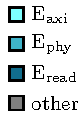
\includegraphics{assets/legend.pdf}
    }
    \hfill
    \subcaptionbox{Excludes states and weight duplicates}{
        \def\printonlylargeenough#1#2{{\unless\ifdim#2pt<#1pt\relax
#2\printnumbertrue
\else
\printnumberfalse
\fi}}
\newif\ifprintnumber

\begin{tikzpicture}
    \pie[
        radius=2.3,
        text=pin,
        hide number,
    ]{
        0.6/0.6\%,
        8.8/8.8\%,
        2.5/2.5\%,
        1.5/1.5\%
    }
    \pie[
        radius=2.3,
        hide number,
        color={gray, bluehue2, bluehue4, bluehue6},
        before number=\printonlylargeenough{2},
        after number=\ifprintnumber\%\fi
    ]{
        0.6/,
        8.8/,
        2.5/,
        1.5/
    }
    \pie[
        radius=1.8,
        text=inside,
        color={blue!60, red!60},
    ]{
        13.5/$\econf$,
        86.5/$\eproc$
    }
\end{tikzpicture}
    }
    \caption{ResNet-50 states and weight duplicates. Based on LPDDR5X as external memory}
    \label{fig:pies_resnet50_no_states_and_dupes_lpddr5x}
\end{figure}
